\chapter{Introducción específica} % Main chapter title

\label{Chapter2}

%----------------------------------------------------------------------------------------
%	SECTION 1
%----------------------------------------------------------------------------------------
En el presente capítulo se describen los componentes de hardware, software y herramientas utilizados para realizar el proyecto.

\section{Estructura del sistema}

En las siguientes secciones se describe la estructura del sistema, con un enfoque en los sistemas embebidos, la detección de objetos y el prototipo desarrollado.

\subsection{Los sistemas embebidos}

En el contexto de la agricultura moderna, los sistemas embebidos se diseñaron para la ejecución de tareas específicas en tiempo real. En el caso del prototipo desarrollado, el sistema se compuso de una serie de módulos, entre ellos cámaras, sensores, pantallas y unidades de almacenamiento. 

Este pudo montarse en un medio de transporte adaptado a las características de la plantación, lo que permitió la captura automatizada de imágenes de los frutos, así como el registro de datos ambientales relevantes durante el recorrido. Toda la información recolectada se almacenó de forma local en una tarjeta microSD, lo que posibilitó su uso de manera independiente de la cobertura de señal.

\subsection{Detección de Objetos}

La detección de objetos constituye una técnica avanzada de visión por computadora que permite identificar y clasificar elementos presentes en las imágenes. Esta tecnología ha demostrado ser particularmente valiosa en el ámbito agrícola, donde la estimación de la producción y la gestión eficiente de los recursos resultan esenciales \citep{Lim2020}.

Para garantizar un funcionamiento correcto de la detección de objetos, se requiere un conjunto de imágenes de entrada. Posteriormente, estas se procesan mediante algoritmos de visión por computadora, que analizan cada entrada con el fin de identificar y contabilizar los frutos \citep{Montiel2019}.

Por otra parte, la detección de objetos se fundamenta en técnicas avanzadas, como el análisis de imágenes y el aprendizaje automático, que permiten diferenciar entre frutos maduros, inmaduros y otros elementos presentes en la plantación.

\newpage

\subsection{El prototipo SIVIC}

El prototipo desarrollado, a partir de ahora denominado SIVIC (Sistema de Visión para Cultivos), está conformado por tres partes esenciales que permiten llevar a cabo su labor. Estas son:
\begin{itemize}
\item El nodo sensor: esta es la parte física o hardware del sistema, utilizado para adquirir las imágenes de la plantación.
\item El firmware: este abarca la lógica del sistema y se encarga de la adquisición, procesamiento y la gestión del almacenamiento de datos. Puede funcionar sobre un sistema operativo de tiempo real o no.
\item El modelo de detección de objetos: este permite realizar la contabilización de los frutos encontrados en las imágenes proporcionadas como entrada.
\end{itemize}

\section{Componentes principales de hardware}

En esta sección se describen en detalle los componentes de hardware y software seleccionados para este trabajo, que resultaron clave para garantizar el funcionamiento de SIVIC.

\subsection{Plataforma de desarrollo STM32 Nucleo-F429ZI}
\label{subsec:F429ZI}

La placa STM32 Nucleo-F429ZI, posee un núcleo ARM Cortex-M4. Esta placa ofrece una plataforma flexible para desarrollar aplicaciones embebidas, con una amplia variedad de interfaces y periféricos, como ADC, DAC, GPIO, SPI, I2C, USART, entre otros. Además, cuenta con compatibilidad con los ecosistemas Arduino y ST Morpho, lo que facilita la expansión y el prototipado rápido. Es ideal para proyectos que requieren procesamiento en tiempo real, gestión de múltiples tareas y alto rendimiento \citep{WEBSITE:Itt2024}.

\subsection{Sensor de temperatura y humedad DHT11}
\label{subsec:dht11}

Este dispositivo, se utiliza para medir temperatura y humedad en ambientes controlados. Es altamente popular debido a su bajo costo y facilidad de uso. Dispone de un sensor capacitivo para medir la humedad y un termistor para la temperatura. El DHT11 proporciona lecturas de humedad en un rango del 20\% al 90\% con una exactitud de ±5\%, y de temperatura entre 0 °C y 50 °C con una precisión de ±2 °C. Se comunica mediante una señal digital, lo que lo hace ideal para aplicaciones en sistemas embebidos y proyectos medianos \citep{WEBSITE:Dht112024}.

\subsection{Display LCD}
\label{subsec:DisplayLCD}

Esta pantalla, capaz de mostrar hasta 16 caracteres en 2 filas, Se utiliza en proyectos de electrónica y sistemas embebidos debido a su simplicidad. Cada carácter se forma a partir de una matriz de puntos de 5 x 8 píxeles, lo que permite visualizar letras, números y símbolos. El display es compatible con microcontroladores y microprocesadores, y se controla mediante interfaces paralelas o serie. Resulta ideal para mostrar información básica, como datos de sensores, mensajes o indicadores de estado en tiempo real \citep{WEBSITE:lcd2024}.

\subsection{Cámara Ov7670}
\label{subsec:camara}

Este módulo compacto de captura de imágenes, mostrado en la figura \ref{fig:camara2024}, se utiliza en proyectos de visión por computadora y sistemas embebidos. El sensor de imagen CMOS Ov7670 puede capturar imágenes en resolución VGA (640x480) y CIF (352x288), lo que lo hace adecuado para aplicaciones de procesamiento de imágenes, seguimiento de objetos y reconocimiento de patrones. La cámara se conecta a microcontroladores o plataformas de desarrollo como Arduino y STM32 mediante interfaces I2C o SCCB para configuración, y una interfaz de datos paralela para la transferencia de imágenes. Además, el módulo ofrece control automático de exposición, balance de blancos y eliminación de ruido, lo que garantiza imágenes de calidad en diversas condiciones de luz \citep{WEBSITE:camara2024}.

\begin{figure}[htbp]
	\centering
	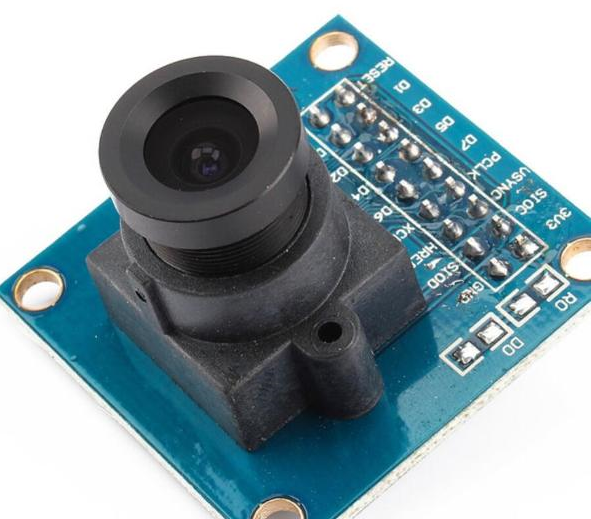
\includegraphics[width=.5\textwidth]{./Figures/camara.png}
	\caption{Cámara Ov7670\protect\footnotemark.}
	\label{fig:camara2024}
\end{figure}

\footnotetext{Imagen tomada de \url{https://www.arcaelectronica.com/products/modulo-de-camara-ov7670-arduino?srsltid=AfmBOopgmnm_0gtPYtNMaSrCGCOKnXMwbjdXpUfh84WJ_Hi9V3akPCPp.}}

\subsection{Sensor ultrasónico HC-SR04}
\label{subsec:hcsr04}

Este dispositivo, se utiliza para medir distancias en proyectos de robótica, sistemas embebidos y automatización. Emite ondas ultrasónicas que se reflejan en objetos cercanos y luego las capta el sensor. El tiempo que tarda la señal en regresar permite calcular la distancia al objeto. El HC-SR04 ofrece un rango de medición de 2 cm a 4 m, con una precisión de aproximadamente 3 mm. Se integra fácilmente con microcontroladores como Arduino o STM32 mediante un sistema de disparo y recepción de señal. Es ideal para aplicaciones como evitar obstáculos, medir niveles de líquido y sistemas de detección de proximidad \citep{WEBSITE:hcsr2024}.

\section{Herramientas de software y testing utilizados}

Las herramientas de software seleccionadas para este trabajo fueron fundamentales para el desarrollo y las pruebas de SIVIC. A continuación se describen en detalle las características principales y los casos de uso de cada una.

\subsection{STM32 CubeIDE}
\label{subsec:stm32}

El sistema STM32 CubeIDE es un entorno de desarrollo integrado (por su sigla del inglés, IDE) creado por STMicroelectronics para trabajar con microcontroladores STM32. Basado en Eclipse, STM32 CubeIDE permite a los desarrolladores escribir, compilar y depurar código en lenguajes como C y C++ y por lo tanto facilita el desarrollo de aplicaciones embebidas. También integra herramientas como STM32CubeMX, que configura los periféricos del microcontrolador y genera código automáticamente \citep{WEBSITE:stm32}.

\subsection{Sistema operativo FreeRTOS}
\label{subsec:FreeRTOS}

Es un sistema operativo en tiempo real (RTOS) de código abierto, ampliamente utilizado en el desarrollo de aplicaciones embebidas. Diseñado para microcontroladores y sistemas de baja potencia, FreeRTOS ofrece un \textit{kernel} ligero y eficiente para gestionar tareas concurrentes de manera óptima. Soporta características clave como multitarea, gestión de memoria, sincronización y temporización precisa, lo que lo convierte en una solución ideal para aplicaciones que requieren control del tiempo y recursos limitados \citep{WEBSITE:freertos}.

\subsection{Pruebas en CEEDLING}
\label{subsec:CEEDLING}

Es una herramienta de testing para proyectos en lenguaje C, diseñada para facilitar el desarrollo y la prueba de software embebido. Este marco de pruebas automatizado proporciona un entorno completo para la creación, ejecución y gestión de pruebas unitarias.

Ceedling integra varias herramientas esenciales para el testing, como CMock, un generador de mocks que simula dependencias y facilita el aislamiento de unidades de código durante las pruebas. Además, utiliza Unity, un framework de pruebas unitarias para C, que ofrece una serie de aserciones y macros para verificar el comportamiento del código.

Además, soporta la ejecución de pruebas en diferentes entornos, genera informes de cobertura de código y facilita la identificación de errores y defectos en el software \citep{WEBSITE:CEEDLING}.

\subsection{Etiquetado de imágenes}
\label{subsec:etiquetado}

El proceso de etiquetado de imágenes resulta fundamental para la construcción de conjuntos de datos en visión por computadora. Consiste en asignar información semántica a cada imagen, de manera que un modelo de aprendizaje automático pueda reconocer y clasificar objetos de interés en futuras inferencias. Entre las herramientas más utilizadas en este ámbito se destacan LabelImg y Roboflow.  

LabelImg es un programa de código abierto diseñado para generar anotaciones en imágenes mediante cuadros delimitadores (\textit{bounding boxes}). Estas anotaciones permiten indicar al modelo qué objeto se encuentra en cada región de la imagen, lo que constituye la base del entrenamiento supervisado. La herramienta es compatible con sistemas operativos Windows, Linux y macOS, y exporta los resultados en formatos ampliamente utilizados, como Pascal VOC (XML) o YOLO (TXT) \citep{WEBSITE:LabelImg}. Su uso resulta especialmente apropiado cuando se dispone de un conjunto propio de imágenes y se requiere preparar los datos para entrenar un modelo desde cero.  

Roboflow, por otra parte, ofrece una plataforma en línea que facilita la gestión integral de conjuntos de datos para visión por computadora. Permite cargar imágenes, generar anotaciones directamente desde el navegador y aplicar técnicas de aumento de datos (\textit{data augmentation}), tales como rotación, recorte o modificación del brillo. Además, la plataforma admite la exportación de los conjuntos de datos en múltiples formatos estándar (YOLO, TensorFlow, COCO, entre otros) \citep{WEBSITE:Roboflow}. Roboflow también brinda la posibilidad de entrenar modelos en la nube y realizar pruebas preliminares, lo que la convierte en una solución flexible y accesible para proyectos de distinta escala.  

\subsection{Modelo de visión por computadora}
\label{subsec:YOLO}

El modelo YOLO (\textit{You Only Look Once}) es un algoritmo avanzado de visión por computadora utilizado en la detección y localización de objetos en imágenes y secuencias de video. Su funcionamiento consiste en dividir la imagen en una cuadrícula y, en una única pasada de la red neuronal, predecir simultáneamente las coordenadas de los cuadros delimitadores (\textit{bounding box}) y las probabilidades de pertenencia a una clase específica (por ejemplo, persona, automóvil o animal) \citep{WEBSITE:YOLO}.

A diferencia de otros enfoques basados en etapas secuenciales de detección y clasificación, YOLO ejecuta ambos procesos de manera conjunta, lo que le confiere alta eficiencia computacional y una velocidad de procesamiento mayor. Estas características lo han consolidado como una herramienta de referencia en tareas que requieren análisis en tiempo real, tales como la conducción autónoma, los sistemas inteligentes de videovigilancia y la navegación asistida por drones.

\section{Protocolos de comunicación}

En el diseño de SIVIC, los protocolos de comunicación cumplen un papel esencial en la interacción entre los distintos componentes del sistema. Entre ellos, UART se basa en una comunicación asíncrona, lo que significa que no requiere una señal de reloj compartida entre los dispositivos que se comunican. En su lugar, utiliza parámetros de configuración como la velocidad de transmisión (\textit{baud rate}), la paridad, el número de bits de datos y el número de bits de parada para sincronizar la transmisión y recepción de datos. \citep{WEBSITE:uart}.

I2C, por otra parte, ofrece una solución versátil para la comunicación entre múltiples dispositivos en el sistema. Utiliza dos líneas para la transmisión de datos: la línea de reloj (SCL) y la línea de datos (SDA). La línea SCL sincroniza la comunicación mediante la señal de reloj, mientras que la línea SDA transporta los datos entre los dispositivos conectados. Ambos hilos son bidireccionales, lo que permite que tanto el maestro como el esclavo envíen y reciban información. \citep{WEBSITE:i2c}.
